\pagestyle{IHA-fancy-style}
\lhead{\textsf{Chapter III}}
\rhead{\textsf{Structural Bioinformatics of PVC Proteins}}


\chapter{Structural Bioinformatics of PVC Proteins}\label{structbioinfo}
\epigraph{\emph{``It is very easy to answer many of these fundamental biological questions; you just look at the thing!''}}{\textit{Richard P. Feynman}}

\section{Introduction}



\todo[inline]{Make a high-level chart of whether genes are more like phage or T6ss e.g. T4Like <------- PVC1           ----------> T6SS}

As large multi-partite biological complexes, there are far too many proteins involved in the biology of PVCs to study them all in detail experimentally within a single project. However, due to the increasing availability of high performance computing resources, it is possible to study all the genes and proteins, to some extent and to reasonable confidence, using bioinformatics approaches. This chapter attempts to glean as many clues as possible about structure and function of the proteins involved in construction of PVCs, by `brute force', but in the application of techinques which have not been attempted to date.

Since there are numerous PVC operons that have been identified, and each one contains $>$16 proteins, the dataset quickly becomes unmanageable for the experimentalist. A rigorous exploration of the hypothetical structures and functions of the proteins can collapse this dataset somewhat, and reveal subtleties of the structures which are interesting or relevant for further study. 

As the databases for gene function and protein structure are continuously updated and improved, this chapter is also a `revisit' to the now outdated genome annotations that were first put together when the strains were sequenced. By re-running these analyses at various points, new putative functions and homologies may be discovered.

Furthermore, this chapter is intended to `pull double duty' somewhat; to serve both as an exploration of new roles and information regarding PVC proteins, but also as a continued, extended, introduction or `guided tour', including what is known about each of the individual proteins within the PVCs, in a similar manner to the exploration of related structures in the Introduction. Hopefully, therefore, this chapter will provide the reader with a understanding of the PVCs with regard to what is already known and what has been discovered, on an almost gene-by-gene basis.

\subsection{The sequence identity problem}
Despite progress in the elucidation of many related structures, as shown in \vref{intro}, much is still unclear with regard to PVCs. Many PVC proteins in the existing \Pa{} annotations are listed as `hypothetical', and in the case of some older genome annotations for some of the more diverse PVC elements, this can be the entire operon \citep{Duchaud2003}. The frequent lack of known good homologues from studying the genes through BLAST for instance, and the degree of sequence diversity that can be seen in the PVCs (see \vref{bioinformatics} for a more in-depth discussion), despite producing the same structure, suggested that structural studies might offer additional/better information.

It is now a widely accepted phenomenon that sequence identity cannot provide sufficient structural understanding on its own, as the evolutionary rules that constrain structures are not exactly the same as those that constrain sequences. Consequently, protein structures are known to evolve slower than the amino acid sequence, and slower still than the nucleotide sequence. In fact, this rate of change has even been quantified, and is estimated to be between three and ten times as slow \citep{Illergard2009}. Moreover, proteins with entirely unrelated sequences can give rise to functionally equivalent proteins, meaning this analogy between proteins would be completely missed through sequence studies alone. Now, of course this does not completely devalue the position of the sequence in determining protein structure and function, however, as \cite{Illergard2009} and \cite{Chothia1986} explain, the relationship between structural similarity (as quantified by Root Mean Square Deviation (RMSD)), and sequence identity is not linear. One of the earliest papers to explore this disconnect defined a so-called `twilight zone' of structural similarity, observing that once sequence identity dropped to around 25\% and below, false positive hits predominate \citep{rost1999twilight}. Just to labor the point a little further, \cite{Holm1996} explain how structures are able to remain much the same, ``even when all sequence memory appears
to have been lost". This means that for proteins whose common ancestors are extremely far back in time, it effectively becomes meaningless to compare the DNA or amino acid sequences, and only the 3D structure matters. The authors summarise this quite nicely with the analogy, 

\begin{displayquote}
``Comparing protein shapes rather than protein sequences is like using a bigger telescope that looks farther into the universe. and thus farther back in time, opening the door to detecting the most remote and most fascinating evolutionary relations."
\end{displayquote}

To change tack for a moment, there are additional issues with sequence identity based analyses which many probably do not fully appreciate - biology is up to its usual tricks once again. Even proteins which \emph{do} share significant sequence identity, do not necessarily have the same structure, and therefore may differ in function. A really good example of this is epitomised by the ``Paracelsus challenge". Posed by \cite{Rose1994}, the challenge was to convert one protein's conformation in to that of another protein by altering less than 50\% of the sequence. This was achieved first by \cite{Dalal1997} (winning them a \$1,000 wager in the process), and though they did have to change roughly 44\% of the protein and include an additional 7 amino acids for solubility, they were able to convert an almost entirely $\beta$-sheet protein in to an entirely $\alpha$-helical one. Subsequently, their effort has been bested by the work of \cite{Alexander2007}, and thoroughly hammers home the message of ``sequence $\neq$ structure". They were able to convert domains from \emph{Streptococcus} G proteins to retain 88\% sequence identity, yet to change their fold structures, all the while keeping their ligand binding activities.

In short, there is no substitute for being able to \emph{see} the tertiary structure and individual folds for each and every protein. This is far from a solved problem however, as it currently requires exhaustive computation and experimental efforts to generate this kind of data. Protein structure simulation has advanced significantly, but is not without its flaws, and of course, the lottery that is protein structure determination via crystallography for example is an incredibly intensive process with a high failure rate. 


Finally, to underscore this idea with some relevant examples, \cite{Leiman2010} observed that ``evolutionary relationships cannot be detected in their [tailed phages] amino acid sequences", but many structural proteins of phage origin share tertiary structure folds. One rationale for this is that given the high turn over rate of phage genomes, their evolution will occur rapidly, and thus they will explore the `chemical space' rapidly also. This is combined with the fact that phages experience a multitude of evolutionary pressures, and being proteinacious entities only, they have to be particularly `inventive' when it comes to protein structure robustness. A further example from the same paper concerns the structures of the VgrG spike proteins. They are often structurally very well conserved which is usually immediately apparent on visual inspection, and yet, the sequences of certain orthologues may share $<$15\% amino acid similarity, and due to redundancy, even lower nucleotide identity. This effectively means that to try and study sequences such as these using sequence data alone would be almost indistinguishable from random noise (though it may be possible to consider small numbers of highly conserved/`privileged' sites).

To make matters even more complicated for purely sequence based studies, for long, multicomponent operons such as the PVCs and other caudate structures, it seems that synteny and gene copy may also be important, potentially playing a role in how the assembly is choreographed (phage early versus late proteins for instance). Papers like that of \cite{Sarris2014}, note that while many of the gene products are identifiable between orthologous operons, the gene copy number varies, as does the syntenic arrangement. In the case of the MAC complex discussed in the first chapter, the whole complex isn't even encoded in one location in the genome \citep{Shikuma2014}. 


To summarise, this chapter looks to address this `conservation of structure not sequence' question with regard to the PVCs, and to infer from these structures in such a way as to provide lab testable hypotheses.

\subsection*{Chapter Aims}

\begin{itemize}
	\item Complete a thorough and sensitive functional annotation of as many PVC proteins as possible.
	\item Generate structural data and compare it to known proteins.
	\item Examine any high quality simulations for physical characteristics of the PVCs.

\end{itemize}

\clearpage

\section{Experimental procedures}
	 A logical first step seemed to be to assess each CDS within 16 PVC operons for any structural similarity (even at comparatively low scores) to glean as much information as possible and form further hypotheses about their roles. Not only does this provide better functional predictions that the existing ones, but simply querying against a more up to date database often turns up previously unseen similarities between proteins.
	 
%    	\subsection{Annotation}\label{annotation}
%    	From a previous project, a number of \Pa{} genomes were sequenced, and a number of existing sequences in NCBI were reassembled and re-annotated along with them for consistency. In all of the work conducted, we utilised the consistent, re-annotated sequences and any given locus tags will correspond to these. Genomes were annotated with a database of existing \Pa{} proteins, utilising Prokka \citep{Seemann2014} (see \vref{methods},  \vref{prokka}).
	
	\subsection{Hidden Markov Model Homology Searching}\label{hhresults}
	As the Protein DataBank and other databases are frequently updated, Hidden Markov Model searches were run repeatedly throughout the course of the project, usually picking up at least 2 or 3 improved structural annotations, with each new run. This was performed using $\mathtt{HHsearch}$ from the HHsuite of tools \citep{Remmert2012}. Searches for 312 proteins were run via a commandline implementation of HHsearch v 2.0.15 on a Ubuntu server, with the following parameters: E-value cutoff = $1\times10^{-3}$, Probability cutoff = 60, and returned the top 10 hits. The searches were queried against the PDB database in each instance, having downloaded the latest version before each run.
	
Hidden Markov Models (``HMMs") are a sensitive way of searching for sequence similarity, that can outperform tools such as BLAST in certain situations. A Markov Model can be thought of as representing each position in the sequence as being one of many different amino acid possibilities, which are weighted. This arise from the fact that not all amino acids are equally likely to appear adjacent to one another - for instance, a stretch of amino acids, all of which can form $\beta$-sheets, are more likely to appear near one another than would an amino acid which contributes to helices, and thus HMMs capture domain information very well. They are suited to the task of identifying distant and very variable homologies, in fact, to quote directly from the HHPred manual: ``HHsearch and HHblits [different algorithm implementations] can detect homologous relationships far beyond the twilight zone, i.e., below 20\% sequence identity. Sequence identity is therefore not an appropriate measure of relatedness anymore."

	
Plot the distribution and use this to highlight the `troublesome proteins'.


"HHsearch and HHblits can detect homologous relationships far
beyond the twilight zone, i.e., below 20\% sequence identity. Sequence identity is therefore not an
appropriate measure of relatedness anymore. "
	
\subsection{Exploration of the structure of PVCs by functional unit}
It has been made abundantly clear that it is insufficient to consider sequence similarity alone when comparing structural proteins. Sequences are at liberty to diverge, and if the structure they give rise to is particularly robust, the `space' that the sequence has to drift in is even larger. This is a generally observed phenomenon, but appears to be particularly true for many of the proteins in contractile tail structres. One postulate for this is that phage represent an extremely ancient domain of life, and spend a significant amount of their life cycle outside of the protective environment of the cell they infect. Thus their proteins have evolved over aeons to become particularly stable and robust. The arms race associated with infection cycles has also no doubt driven the diversification of these proteins in an effort to avoid immune mechanisms of their hosts. It has been observed many times in the related literature that, for example, the vgrG/gp5-gp27 spike complex of these caudate systems look almost identical structurally, with many of the same domains identifiable such as the OB-fold, yet may share as little as 12\% protein sequence identity, and due to the slower evolution of proteins sequences attributable codon redundancy, the corresponding DNA sequences may be even less similar.

Consequently, we must make efforts to study the structure as best as possible. In silico methods are improiving all the time, and with more computer power than ever, simulations are becoming routinely feasible. threading approaches are not ideal as they are still too dependent on first identifyin sequence similarity. ab initio approaches allow the structures to be refined without a dependence on the sequence, which should offer an improvement. Structurally conserved proteins with a high degree of robustness should therefore naturally coalesce toward the same structure.

\subsection{The PVC tube}
\addfloat{Image of PVC1-5 in locus position}
Among the better annotated genes at the outset of this work, the first 5 loci of the PVCs, are predicted to match phage tail tube proteins, though the existing annotations were not much more informative than this (the vast majority of which were ``hypothetical proteins"). After re-annotation, these genes are consistently annotated as T4-like virus tail tube or baseplate proteins (orthologs of gp6/gp19) and sheath proteins from the recently resolved \emph{Pseudomonas aeruginosa} R-type pyocin. From the resolved structure databases and literature, gp19 is known to be the inner sheath of the T4 bacteriophage (as can be seen in PDB IDs 5IV5 and 5W5F \citep{Taylor2016, Zheng2017}), and the outer sheath of PDB ID 3J9Q which corresponds to the resolved pyocin tube structure \citep{Ge2015a}. Over several iterations of homology searches with the HHpred suite, these 3 recent PDB depositions have come to be the most highly similar structures predicted, though in past results, the best hits have included Type 6 Secretion System components from \emph{Edwardsiella tarda} (for the outer sheath proteins).

These proteins comprise the bulk of the PVC, with electron microscopy estimates suggesting that they are about 200 nm in length, and therefore probably include as many as 50 hexameric `donuts' of each, taking in to account the measurements in \vref{tubestructure}


The upcoming figures demonstrate the simulated structure similarities to the published known structures. In each case, as there are up to 5 simulated models per locus, and up to 16 alleles, so for simplicity, the `best' model, from the best fitting is, and an conservation map by overlaying the multiple sequence alignments in \ref{bioinformatics_appendix}  to encapsulate the variability, as well as a strucuture overlay.

For the outer sheath, there are 3 loci, for there are 1 loci, so each of these are shown separately



Interior sheath proteins are smaller but much better conserved. This is suggestive of photorhabdus honing the exterior of the sheath in different environments.

\clearpage
\begin{figure}[h!]
{\centering
    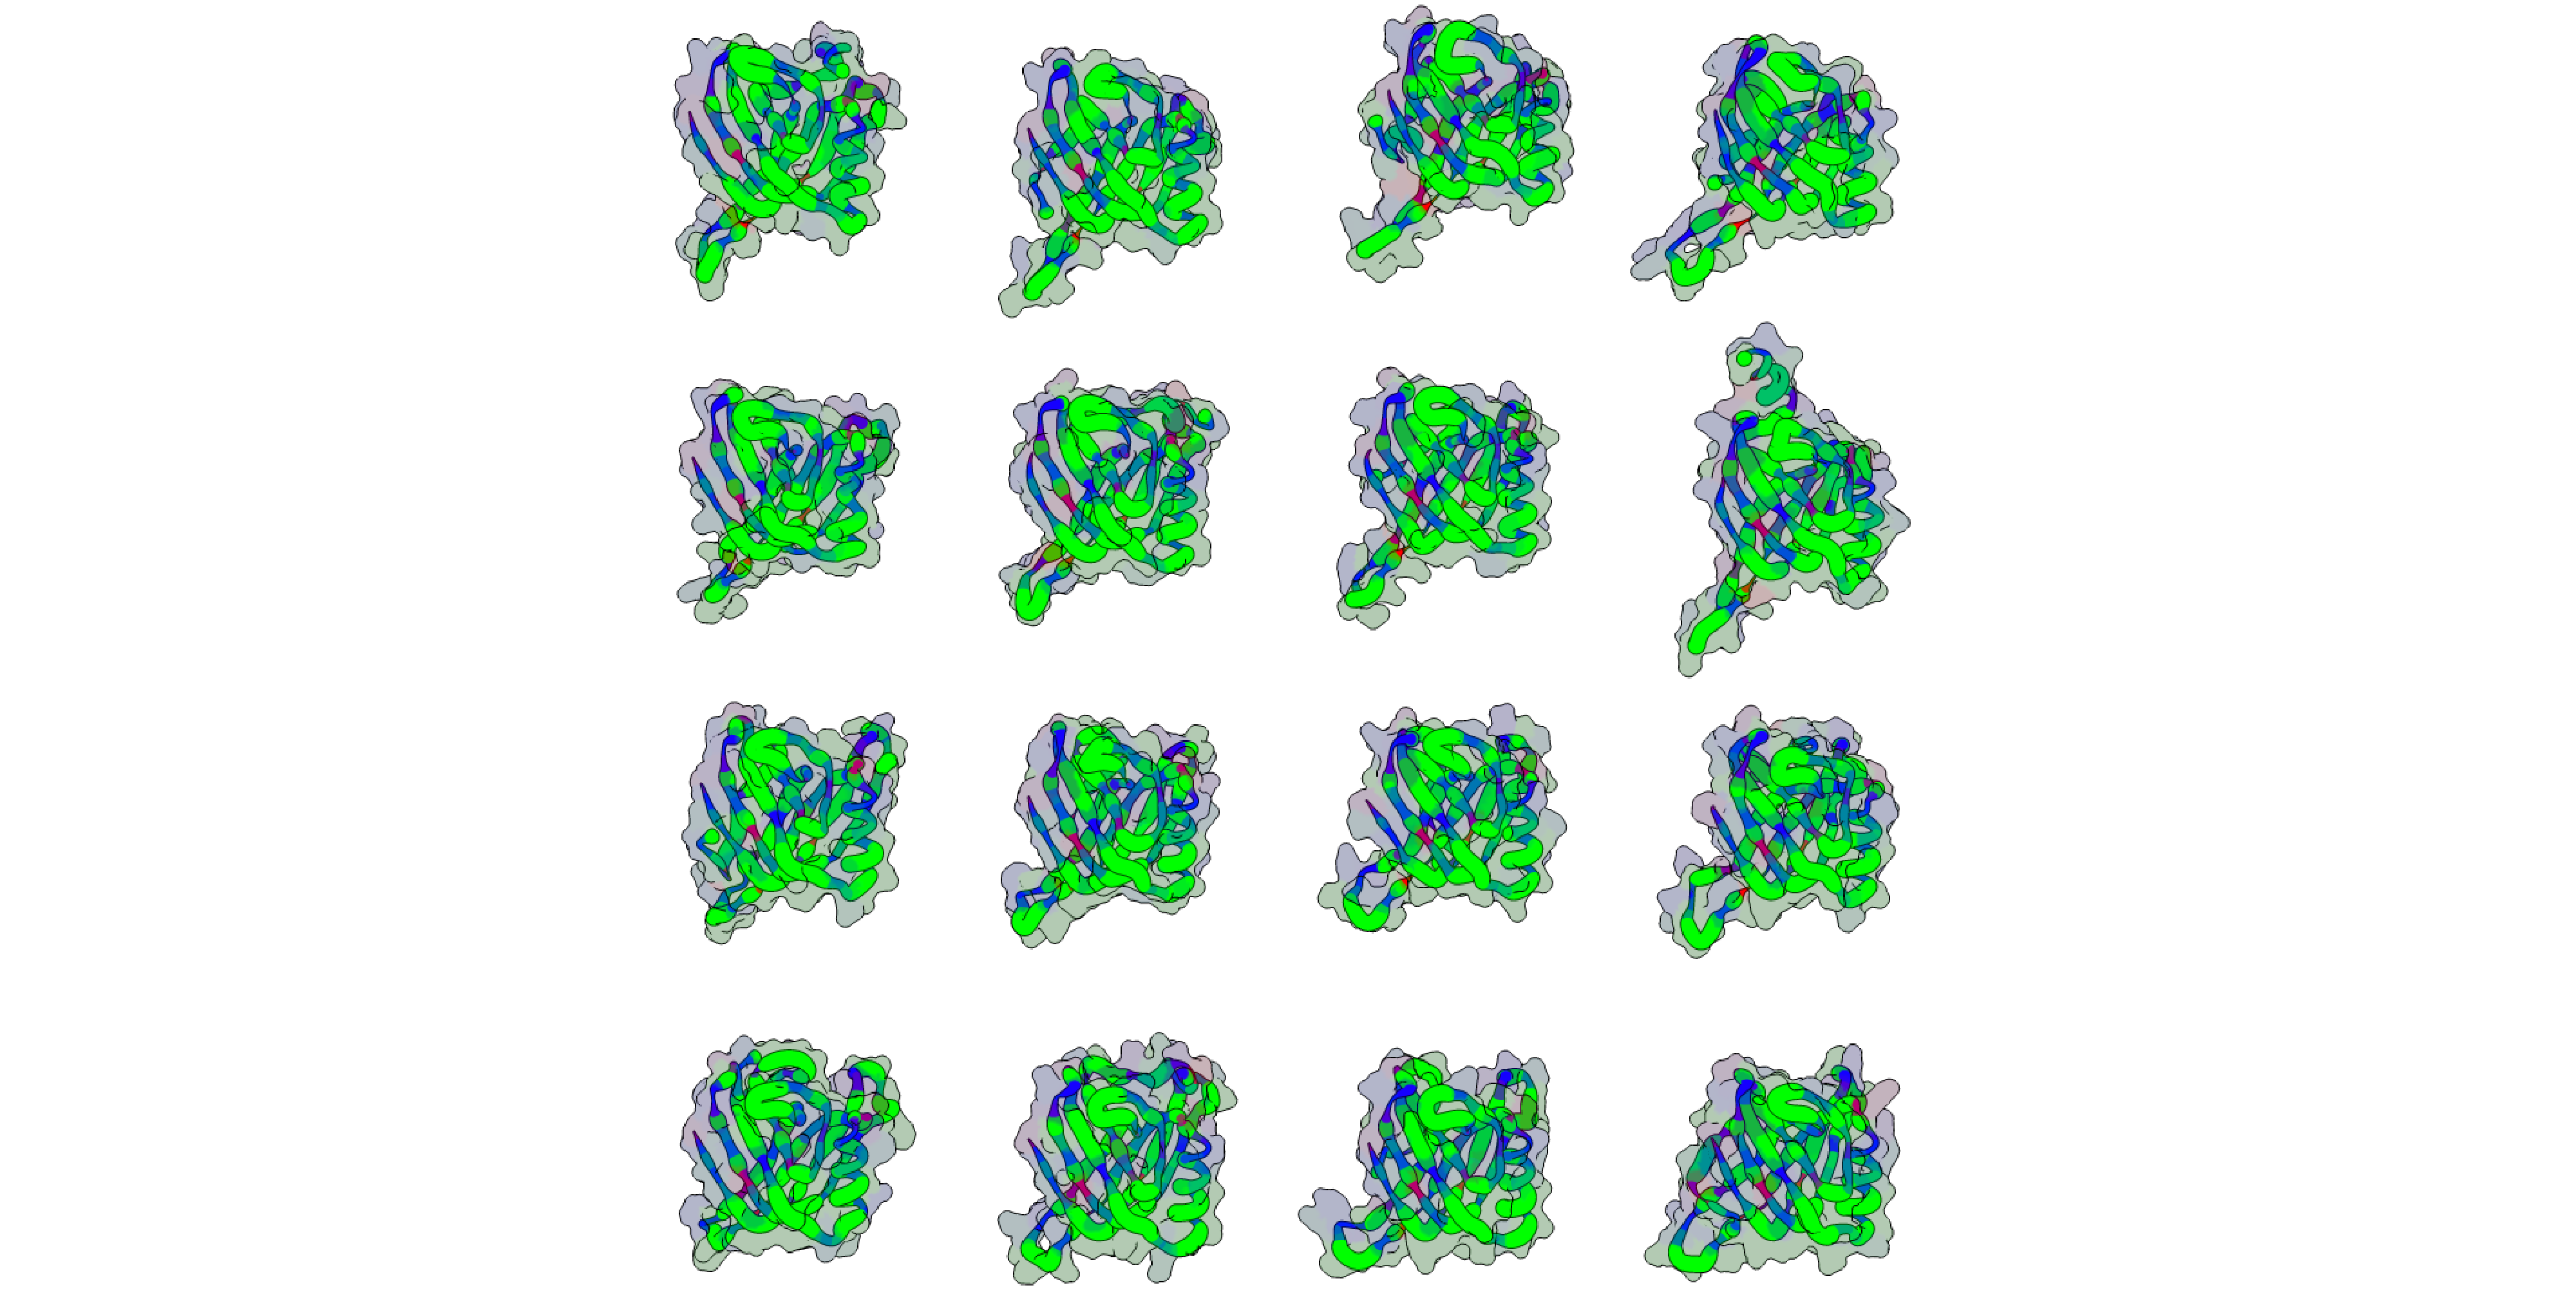
\includegraphics[width=\textwidth, clip, trim={490 0 490 0}]{/Users/joehealey/Documents/Warwick/PhD/Thesis/chapters/chapter3/img/PVC1_conservations.pdf}
}


\includegraphics[width=0.1\textwidth, clip, trim={0 0 0 0}]{/Users/joehealey/Documents/Warwick/PhD/Thesis/Thesis_Scaffold/Auglogo.png}

\end{figure}
\clearpage

\addfloat{Immunogenicity profiling of exterior sheath}
\addfloat{Electrostatic comparisons of interior tube proteins + general comparisons}
\addfloat{comparisons of PVCs2,3,4 to try and understand their paralogy?}



\addfloat{table of HHpred matches}























\section{Discussion}
PVCs are a hybrid between T4 and pyocin like structures, with an inner sheath most resembling the former, and an outer sheath the latter.




\todo[inline]{Table of HHpred results in appendix}
\todo[inline]{Correlation between sequence similarity and structure similarity}




